\documentclass[11pt]{article}
\usepackage[margin=1.1in]{geometry}
\usepackage[T1]{fontenc}
\usepackage{lmodern}
\usepackage{microtype}
\usepackage{array}
\usepackage{longtable}
\usepackage{hyperref}
\hypersetup{colorlinks=true, linkcolor=black, urlcolor=blue!50!black}
\usepackage{enumitem}
\setlist{nosep}
\usepackage{tikz}
\usetikzlibrary{positioning,arrows.meta,shapes.geometric}

\title{A Capability Proof, by Construction:\\
\large Automated theorem-proving on a qualifying-exam corpus,\\
with graded warrants and machine-checkable certificates}
\author{Joseph Corneli\thanks{Prepared with the futon agent mesh
(Claude, Codex, and Z.ai seats coordinated over a local Agency);
the human's role was direction, review checkpoints, and the
judgments marked as such below.}}
\date{4 August 2026 --- working note, v1}

\newcommand{\node}[1]{\textbf{#1}}
\newcommand{\warrant}[1]{\textsl{#1}}

\begin{document}
\maketitle

\begin{abstract}\noindent
We are formalizing and solving a corpus of ${\sim}493$ mathematics
qualifying-exam problems (``APM'') in Lean~4/Mathlib, using a relay of
LLM agents. Rather than reporting a solve rate, we organize the whole
programme as a \emph{proof by construction} of the claim ``all APM
problems are solved'': the constructive content is an automated
pipeline; the claim decomposes into sub-claims (typed holes with
contracts); and each sub-claim carries a \emph{graded warrant} backed
by machine-checkable certificates --- compiler exits, axiom audits,
statement hashes, append-only ledgers --- rather than narrative. The
pipeline closed its first theorem end-to-end under automation
(Steinhaus's theorem) on the day the driver was built. We describe the
method, the current warrant state (including the deliberately weak
nodes), and the causal-inference layer used to keep claims about
\emph{why} components work identified rather than merely correlated.
The intended contribution is less the solve rate than the epistemic
form: a research programme whose own capability claim is held to the
same standard of proof as its object-level theorems.
\end{abstract}

\section{The claim, read constructively}

The headline claim --- \emph{all APM problems are solved} --- is
false today (${\sim}27\%$ of the corpus is closed) and will not be
proved by enumeration. Read constructively (in the
Brouwer--Heyting--Kolmogorov sense), the claim asserts instead that a
\emph{procedure} exists which, handed any APM problem, produces a
mechanically-verified solution --- together with witnesses that each
component of the procedure does its job. The proof object is the
pipeline; the corpus percentage is merely its odometer.

This reading changes what counts as progress. Evidence attaches to
\emph{components} (sub-claims), each stated with a contract and a
current warrant; the top-level claim is discharged when the component
warrants are strong and the composition runs continuously. The
document that holds this structure is a live file, updated
mechanically by the pipeline itself, under one rule: \textbf{a warrant
upgrades only by certificate, never by narrative.}

\section{Warrants and certificates}

Six warrant classes are in use: \warrant{mechanical} (an executed
witness: the Lean compiler exits 0, the axiom audit is clean, a
statement hash matches); \warrant{replicated} (independent runs agree
on the load-bearing quantities); \warrant{inductive-$n{=}K$} ($K$
observed instances, honesty bounds stated); \warrant{designed}
(contract written, no witnesses yet); \warrant{registered} (candidate
mechanism, not yet applied); and \warrant{refused} --- which
distinguishes \emph{proved-impossible} from \emph{not-yet-capable},
because conflating those two species of ``no'' destroys planning.

Certificates are cheap and adversarial by construction: every code
module was built by one agent and reviewed by another (author
$\neq$ reviewer, enforced in the memory store's attachment lifecycle
as well as in process); every claimed number was re-derived by the
reviewer from the artifacts; mock-confirmed assumptions are
explicitly distrusted after two same-day incidents in which a test
suite faithfully validated its author's invention while the live
system disagreed. Heterogeneous warrants are the point, not a defect:
an honest proof marks precisely where certification is absent.

\section{The construction}

The pipeline is a relay with a division of labour that emerged from
measurement, not doctrine:

\begin{enumerate}
\item \textbf{Starter} (Z.ai seat): reads the informal problem (TeX +
prose), performs a memory-reconnaissance pass over the programme's
evidence store, then formalizes a faithful Lean statement and proves
as far as it honestly can. A partial ends at a \emph{boundary
artifact}: the smallest possible \texttt{sorry} at the exact missing
bridge, with a comment recording APIs searched, routes tried, and
routes \emph{not} investigated.
\item \textbf{Mechanical gate} (no model in the loop): build, a
comment-stripped \texttt{sorry} count, a verbatim \texttt{\#print
axioms} audit, a whitespace-stable statement hash (frozen at first
formalization; any later mismatch voids the chain), and a
boundary-conformance check.
\item \textbf{Closer} (Codex seat, $\le 3$ hops): receives the
boundary artifact and closes the hole --- by finding the missing
lemma, proving it locally, or routing around it. Desk research
(Mathlib source, previously solved neighbours, git history) is
framed as part of the job, with discards recorded with reasons.
\item \textbf{Human-judgment checkpoints, and only these}: fidelity
of a fresh formal statement to its informal source (adjudicated
against the TeX contract), and anomalies. Both arrive as structured
requests with everything needed to adjudicate; verdicts are files;
everything else is automatic.
\item \textbf{Scribe}: after each chain, an extraction pass distills
reviewed memories (lemma locations, reusable proof patterns,
consultation practices) into the evidence store, including a
\emph{hunger audit}: retrieval queries that returned nothing are
recorded as demand signals, and memories answering them carry the
asker's literal vocabulary as tags.
\end{enumerate}

Every transition is a record in an append-only ledger under a
registered identity; state is derived by folding the ledger, illegal
transitions are unrepresentable, and the operator can inspect any
chain at any moment. These properties are requirements extracted from
a failure (an earlier opaque cron dispatcher was retired for exactly
this), not aspirations.

\section{Current warrant state}

\begin{center}
\small
\begin{tabular}{p{0.34\textwidth} p{0.17\textwidth} p{0.38\textwidth}}
\textbf{Sub-claim} & \textbf{Warrant} & \textbf{Key certificates}\\[2pt]
\hline\\[-8pt]
N1 Extra resources fill Mathlib holes & inductive-$n{=}3$ &
interval-decomposition lemma proved locally in ${\sim}15$ min;
Liouville derived without the packaged theorem; L\textsuperscript{1}
translation-continuity bridge found and used (Steinhaus)\\[3pt]
N2 Work transports between agents & inductive-$n{=}4$ & boundary
artifacts paved each closer's path; cross-problem reuse cited in
source; protocol itself stored as a memory\\[3pt]
N3 The store records learning & inductive-$n{=}4$ sessions & 20
reviewed, tagged, attached memories in two days; extraction quality
held without correction; hunger audit ran unattended\\[3pt]
N4 Agents consult memory when instructed & inductive-$n{=}1$
(controlled) & same agent, same store: 0 lookups under a passive
invitation vs.\ 21 under a two-part task frame\\[3pt]
N5 Retrieval serves the need & \textbf{weak} & a four-layer failure
anatomy (propensity / framing / affordance / index-reach) with one
positive instance; repairs identified and queued\\[3pt]
N6 Capability transports to held-out problems & designed & stated as
a formal transportability claim; no witnesses yet\\[3pt]
N7 Outcomes are mechanically scoreable & designed$\to$mechanical &
delta-form endpoint, executed-witness-only scoring; capture landing\\[3pt]
N8 The process learns at the ability level & designed & lessons
travel via versioned packet templates; automation of template deltas
not yet built\\[3pt]
N9 The pipeline runs continuously & inductive-$n{=}2$ chains & driver
built in one day from six independently reviewed modules; supervised
trial witnessed both branches (see below)\\
\hline
\end{tabular}
\end{center}

\medskip
The two trial chains are worth a sentence each, because together they
witness the composition. \textbf{Chain 1} (Dirichlet integral): the
starter session died mid-work at 43 minutes; the gate correctly
refused the corpse; the anomaly checkpoint fired with a complete
dossier; the human verdict (\emph{abandon}) folded on restart; two
instrument defects were found and fixed as a result. The safety
branch works, and failures are data. \textbf{Chain 2} (Steinhaus's
theorem): the starter produced an exemplary honest partial --- the
exact missing bridge documented with APIs searched and routes
untried; a gate false-positive was caught at the checkpoint, the
\emph{instrument} was fixed rather than the artifact, and on resume
the closer supplied the missing continuity bridge
(\texttt{tendsto\_measure\_symmDiff\_preimage\_nhds\_zero}), closing
the theorem: build clean, zero \texttt{sorry}s, axioms exactly
\texttt{[propext, Classical.choice, Quot.sound]}, fidelity
adjudicated against the TeX contract. The scribe then wrote four
memories --- including the programme's first \emph{open-hunger}
record: a query the corpus could not answer, banked as demand.

\section{The causal layer}

\begin{figure}[t]
\centering
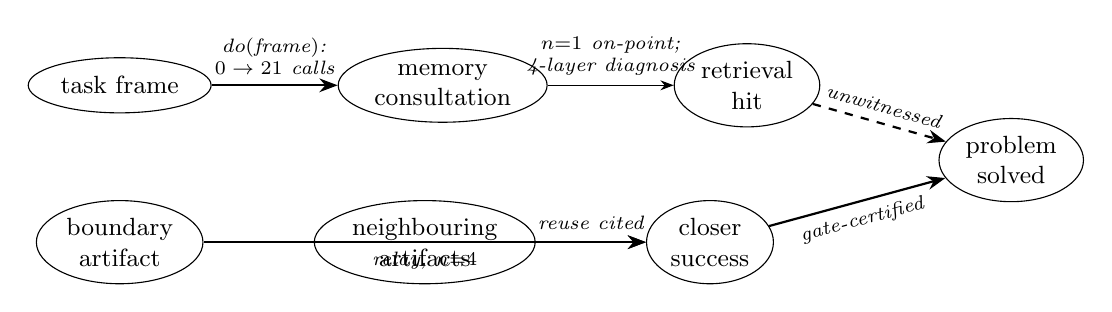
\begin{tikzpicture}[
  every node/.style={font=\small},
  var/.style={draw, ellipse, minimum height=7mm, inner sep=2pt, align=center},
  wit/.style={-{Stealth}, thick},
  unwit/.style={-{Stealth}, thick, dashed},
  lab/.style={font=\scriptsize\itshape, midway, align=center}]

\node[var] (frame) {task frame};
\node[var, right=16mm of frame] (consult) {memory\\consultation};
\node[var, right=16mm of consult] (hit) {retrieval\\hit};
\node[var, below=11mm of frame] (boundary) {boundary\\artifact};
\node[var, right=14mm of boundary] (neighbor) {neighbouring\\artifacts};
\node[var, right=14mm of neighbor] (closer) {closer\\success};
\node[var, right=15mm of hit, yshift=-9.5mm] (solved) {problem\\solved};

\draw[wit] (frame) -- node[lab, above] {$do(\textrm{frame})$:\\$0\to21$ calls} (consult);
\draw[wit, thin] (consult) -- node[lab, above] {$n{=}1$ on-point;\\4-layer diagnosis} (hit);
\draw[unwit] (hit) -- node[lab, above, sloped] {unwitnessed} (solved);
\draw[wit] (boundary) -- node[lab, below] {relay, $n{=}4$} (closer);
\draw[wit] (neighbor) -- node[lab, above, yshift=1pt] {reuse cited} (closer);
\draw[wit] (closer) -- node[lab, below, sloped] {gate-certified} (solved);
\end{tikzpicture}
\hspace{8mm}
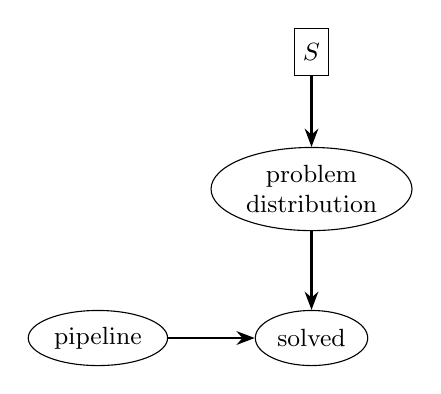
\begin{tikzpicture}[
  every node/.style={font=\small},
  var/.style={draw, ellipse, minimum height=7mm, inner sep=2pt, align=center},
  sel/.style={draw, rectangle, minimum height=6mm, inner sep=3pt},
  wit/.style={-{Stealth}, thick}]
\node[sel] (S) {$S$};
\node[var, below=9mm of S] (dist) {problem\\distribution};
\node[var, below=10mm of dist] (solve) {solved};
\node[var, left=11mm of solve] (pipe) {pipeline};
\draw[wit] (S) -- (dist);
\draw[wit] (dist) -- (solve);
\draw[wit] (pipe) -- (solve);
\end{tikzpicture}
\caption{\textbf{Left:} the mechanism DAG as currently witnessed.
Solid edges carry certificates (labels); the dashed edge is the
honest gap --- retrieval hits have not yet been shown to cause
solutions (every hint so far was correctly discarded as
off-route). The $do(\cdot)$ edge is the programme's one true
intervention: a preregistered controlled contrast on the task
frame. \textbf{Right:} the transport question N6 as a selection
diagram: $S$ switches the problem distribution (APM vs.\ held-out
BPM); the claim ``the pipeline works on BPM'' is identified only if
the $S$-dependence can be separated from the pipeline edge ---
which is a derivation obligation, not an extrapolation.}
\label{fig:dag}
\end{figure}

``The memory system helps'' is a causal claim, and we treat it with
the same discipline as the theorems (Figure~\ref{fig:dag}). Contrasts are designed before
they are run (the $n{=}1$ controlled contrast in N4 was
preregistered, with its predictions written down and two of them
subsequently refuted by the data --- refuted predictions being
exactly what preregistration is for). Identification precedes
estimation: a small causal engine (Pearl-style: backdoor and
front-door adjustment, general identification, transportability via
selection diagrams) supplies receipts for which contrasts are
identified by design and refuses the rest; N6 above is stated in its
vocabulary because ``solves APM $\Rightarrow$ capable on held-out
BPM'' is formally a transport claim, not an induction. Where evidence
is observational or $n$ is small, the warrant says so; nothing in
the table above launders correlation into mechanism.

\section{Honest boundaries}

N5 is weak and is named as the binding constraint on the memory loop:
agents now reliably \emph{ask} (N4), but the store does not yet
reliably \emph{answer}, for reasons diagnosed to the index and
affordance layers, with mechanical repairs queued. N6 has no
witnesses. The corpus is ${\sim}27\%$ closed and the inductive $n$'s
are small everywhere --- the table is a statement of what has been
witnessed, not of what is expected. Two structural findings temper
optimism about memory in particular: within a relay chain, the
\emph{repository itself} (boundary comments, neighbouring solved
problems) has so far been the memory channel that demonstrably works;
the store's value is amortized \emph{across} chains and is only now
becoming measurable. And instructions dominate architecture at every
margin measured so far: one plain sentence of task framing moved
memory-tool usage from zero to twenty-one calls.

\section{What this is for}

The pipeline will keep eating the corpus, and the live document will
keep upgrading warrants by certificate. But the transferable object,
we think, is the form: a research programme that states its own
capability claim as a constructive theorem, decomposes it into
contracted holes, refuses to let anything upgrade without a
machine-checkable witness, and keeps its refusals typed. The same
form is now being applied, by a second agent lane, to a harder
subject: the memory architecture itself.

\end{document}
